\documentclass[a4paper]{article}

\usepackage[utf8]{inputenc}
\usepackage[portuges]{babel}
\usepackage{indentfirst}
\usepackage{graphicx}
\usepackage{float}
\usepackage{caption}
\usepackage{subcaption}
\usepackage[T1]{fontenc}
\usepackage{listings}
\usepackage{amsmath}
\usepackage{mathtools}
\usepackage{courier} %% Sets font for listing as Courier.
\usepackage{listings, xcolor}
\lstset{
tabsize = 4, %% Sets tab space width.
showstringspaces = false, %% Prevents space marking in strings, string is defined as the text that is generally printed directly to the console.
numbers = left, %% Displays line numbers on the left.
commentstyle = \color{green}, %% Sets comment color.
keywordstyle = \color{blue}, %% Sets  keyword color.
stringstyle = \color{red}, %% Sets  string color.
rulecolor = \color{black}, %% Sets frame color to avoid being affected by text color.
basicstyle = \small \ttfamily , %% Sets listing font and size.
breaklines = true, %% Enables line breaking.
numberstyle = \tiny,
}
\renewcommand{\familydefault}{\sfdefault}


\title{Projeto de Computação Gráfica - Fase 4}
\author{Diogo Braga A82547 \and João Silva A82005 \and Ricardo Caçador A81064
\and Ricardo Veloso A81919}
\date{\today}

\begin{document}

\maketitle

\begin{abstract}
Neste relatório é apresentada a quarta fase dum projeto no qual a intenção é desenvolver um mecanismo baseado em gráficos 3D e fornecer exemplos de uso que mostrem o seu potencial. Este projeto é desenvolvido no âmbito da unidade curricular de Computação Gráfica.
\end{abstract}

\newpage

\tableofcontents


\newpage

\section{Introdução}
\label{sec:intro}

Nesta última fase serão feitas as últimas alterações no \textit{Generator} e no \textit{Engine}.


No caso do \textit{Generator} :

\begin{enumerate}
	\item Serão geradas \textbf{coordenadas} para as texturas.
	\item Serão gerados \textbf{vetores normais} para cada vértice com o objetivo de, posteriormente, proporcionar iluminação.
\end{enumerate}

No caso do \textit{Engine} :

\begin{enumerate}
	\item Realizar o parsing do ficheiro XML que irá conter as informações relativas à ilimunição e às texturas e guardar a informação retirada nas devidas estruturas.
	\item Ativar as funcionalidades da iluminação e das texturas.
	\item Aplicar as \textbf{coordenadas} e os \textbf{vetores criados} no \textit{Generator}.
\end{enumerate}

De seguida iremos apresentar figuras, algoritmos e as suas respetivas explicações de forma a ilustrar a realização das etapas apresentadas acima.

\section{Estrutura da Pasta do Projeto}
\label{sec:estrutura}

Para um entendimento mais claro da estrutura do projeto, achamos por bem referenciar a estrutura da pasta do projeto.
O projeto entregue contêm para além do relatório, 4 pastas como é possível verificar na seguinte figura.

\begin{figure}[H]
\centering
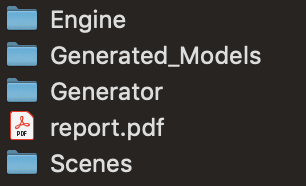
\includegraphics[scale=1.0]{estrutura.png}
\caption{Estrutura da pasta.}
\label{img:estrutura}
\end{figure}

Na pasta \textbf{Scenes} foram inseridas as imagens necessárias para as texturas.

De resto, relativamente à fase anterior não podemos apontar qualquer diferença sendo que não foi acrescentado qualquer ficheiro ou pasta à estrutura do projeto isto porque a quarta e última fase apenas envolve a realização de alterações no código dos ficheiros já existentes.

\newpage

\section{Estruturas de dados}
\label{sec:estruturadados}

No que conta a estruturas de dados há alguns aspetos importantes a abordar.

Foram criadas duas novas estruturas \textbf{TexturePoint} e \textbf{Light}.

\begin{lstlisting}[language = C++ , frame = trBL , firstnumber = 1 , escapeinside={(*@}{@*)}]
	class TexturePoint{
        	public:
           		float x,y;
   	 };
\end{lstlisting}

Esta estrutura serve unicamente para armazenar coordenadas de textura, uma vez que a estrutura \textbf{Point} tem 3 coordenadas e não serve para armazenar uma estrutura que tenha só duas.

\begin{lstlisting}[language = C++ , frame = trBL , firstnumber = 1 , escapeinside={(*@}{@*)}]
	class Light{
        public:
        	GLenum l;
        	float pos[4], amb[4], diff[4];
        	float dir[3];

        	void apply(){
        		glLightfv(l, GL_POSITION, pos);
        		glLightfv(l, GL_AMBIENT, amb);
        		glLightfv(l, GL_DIFFUSE, diff);
        	}
    };
\end{lstlisting}

A estrutura \textbf{Lights} serve para armazenar o número da luz correspondente bem como as suas propriedades.

Contém ainda uma função \textbf{apply()} que ativa os parâmetros da luz em questão.

Para além destas duas estruturas que foram criadas existem outras que foram alteradas como por exemplo a \textbf{Tree}, a \textbf{Figure} e a \textbf{Color}.

 \begin{lstlisting}[language = C++ , frame = trBL , firstnumber = 1 , escapeinside={(*@}{@*)}]
	class Tree{
        public:
            Figure head_figure;
            vector<Tree> children;
            vector<Light> lights;
    };
\end{lstlisting}

Começando pela \textbf{Tree} foi-lhe adicionado um \textbf{vector<Light>} para que armazenasse as luzes presentes na cena.


 \begin{lstlisting}[language = C++ , frame = trBL , firstnumber = 1 , escapeinside={(*@}{@*)}]
	class Figure{
        public:
            Figure(): points(-1){}
            string name;
            int num_triangles;
            int points, normals, textures;
            GLuint textureId;
            Translation translation;
            Rotation rotation;
            Scale scale;
            Color color;
    };
\end{lstlisting}

A estrutura \textbf{Figure} foi remodelada no aspeto em que saíram os \textbf{vector} existentes que armazenavam todos os pontos e normais, para serem trocados por inteiros que representassem o identificador da VBO correspondente.

Foi ainda adicionado o parâmetro \textbf{textureId} que identifica o identificador da textura correspondente.

 \begin{lstlisting}[language = C++ , frame = trBL , firstnumber = 1 , escapeinside={(*@}{@*)}]
	class Color{
        public:
            Color() : diffuseColor(NULL), specularColor(NULL), emissiveColor(NULL), ambientColor(NULL), empty(true){}
	        bool empty;
	        float *diffuseColor,
		          *specularColor,
		          *emissiveColor,
                  *ambientColor;
    };
\end{lstlisting}

Por último a estrutura \textbf{Color} foi totalmente remodelada uma vez que anteriormente era usada apenas para dar cor às figuras geométricas e tinha apenas 3 atributos.

Com a iluminação é necessário que esta estrutura tenha capacidade de armazenar todos os parâmetros relacionados com o material do objeto.

Desta forma apresenta 4 arrays de float que identificam tais parâmetros.



\section{Iluminação}
\label{sec:iluminacao}

\subsection{Generator}
\label{sec:generatori}

Nesta fase, para o funcionamento dos pontos de luz, foi necessário estabelecer as normais dos vértices que formam os triângulos, tanto no caso da esfera (sol, planetas e luas), como no caso do torus (anel de saturno) e da superfície de bezier (cometa). Como os vértices têm coordenadas diferentes, estes possuem também normais diferentes. Quando todas as normais estão disponíveis, a intensidade para cada uma delas é calculada.

O cálculo das normais é realizado tendo em conta os valores dos vértices já definidos. Tendo em conta que os valores das componentes das normais possuem valores entre 0 e 1, estes são calculados reajustando os valores das componentes dos vértices para valores entre 0 e 1. Tal acontece pois a ideia deste método é a normal possuir a direção do vértice.

Todo o restante cálculo dos vértices já tinha sido produzido.

Na figura \ref{img:vertice_normal} é possível visualizar um exemplo de um reajustamento entre um vértice e uma normal.

\begin{figure}[H]
\centering
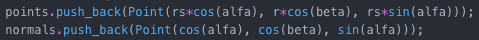
\includegraphics[scale=0.60]{vertice_normal.png}
\caption{Exemplo de vértice e respetiva normal.}
\label{img:vertice_normal}
\end{figure}

\subsection{Parser XML}
\label{sec:parseri}

\subsubsection{Ficheiro}
\label{sec:ficheiroi}

Devido aos requerimentos desta fase foi necessário alterar o ficheiro XML que provinha da terceira fase. As alterações aconteceram devido à necessidade de incluir no ficheiro os pontos de iluminação.

Importante referir que também nesta fase todos os sub-grupos herdam as transformações geométricas presentes no grupo ao qual pertencem. As transformações são: translações, rotações e escalas. O funcionamento é igual à fase anterior.

A definição dos pontos de iluminação baseia-se no tipo de luz, na posição, e nas componentes difusa e ambiente.

Na figura \ref{img:ficheiro_parser_iluminacao} é possível visualizar os quatro pontos de iluminação que estão incluidos na cena.

Os pontos foram colocados próximos do sol nos eixo Ox e Oz, tanto do lado positivo como do lado negativo. Desta forma, é dada a ideia do sol iluminar todos os planetas e luas.

\begin{figure}[H]
\centering
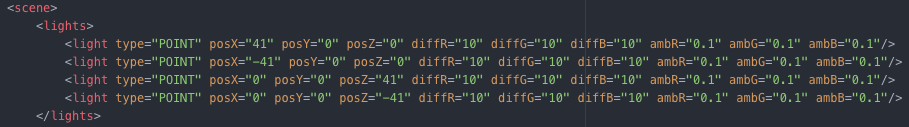
\includegraphics[scale=0.35]{ficheiro_parser_iluminacao.png}
\caption{Pontos de iluminação presentes na cena.}
\label{img:ficheiro_parser_iluminacao}
\end{figure}

\subsubsection{Funcionamento}
\label{sec:funcionamentoi}

Tendo em conta as alterações referidas no ponto anterior, foi necessário acrescentar ao \textit{parser} a capacidade de processar os pontos de luz. Tal ocorre da seguinte forma:

\ttfamily
\begin{enumerate}
  \item Executa a função "parser\_Lights" que vai colocar na estrutura de dados as luzes.
  \item Para cada ponto de luz:
  \begin{enumerate}
    \item Obtém o valor do tipo de luz.
		\begin{enumerate}
			\item Consoante o tipo, altera a direção da luz (último parâmetro).
		\end{enumerate}
		\item Obtém o valor da posição.
		\item Obtém o valor da componente ambiente.
		\item Obtém o valor da componente difusa.
		\end{enumerate}
  	\item Retorna as luzes, que vão ser colocadas na estrutura.
\end{enumerate}
\rmfamily


\subsection{Engine}
\label{sec:enginei}

No ciclo de rendering, os parâmetros das luzes são estabelecidos através da função \textbf{glLightfv}, nas três componentes: Posição, Ambiente e Difusa.

Na função \textbf{initGL}, as luzes são ativadas através da função \textbf{glEnable}.

Desta forma, conseguimos implementar iluminação e todas as suas variáveis no sistema solar.

\section{Texturas}
\label{sec:texturas}

\subsection{Generator}
\label{sec:generatort}

No \textbf{Generator} foram alteradas apenas as figuras geométricas que foram necessárias para utilizar no sistema solar, respetivamente a \textbf{sphere} (sol, planetas e luas), o \textbf{torus} (anel de saturno) e por último a \textbf{superfície de bezier} (cometa).

Nesta fase iremos explicar o procedimento realizado para esfera sendo que para as outras figuras geométricas seguiram um raciocínio semelhante.

\subsubsection{Algoritmo}
\label{sec:algoritmot}

\ttfamily
\begin{enumerate}
  \item Define-se o tamanho de partição da imagem consoante as slices e as stacks:
   	$$deltaS = \frac{1}{slices}$$  $$deltaT = \frac{1}{stacks}$$
  \item Para cada stack:
  \begin{enumerate}
  	\item Define-se a coordenada da stack atual
	$$ t = (stacks - i) \times deltaT $$
	\item Para cada slice:
	\begin{enumerate}
	 	\item Define-se a coordenada da slice atual
		$$ s = j \times deltaS $$
		\item Desenham-se as coordenadas para os 2 triângulos
	\end{enumerate}
  \end{enumerate}
  \item Coordenas são guardadas em ficheiro intercaladas com os pontos e as normais
\end{enumerate}
\rmfamily


\subsection{Parser XML}
\label{sec:parsert}

\subsubsection{Ficheiro}
\label{sec:ficheirot}

Uma textura é dada pelo nome duma imagem da seguinte forma em XML:

\begin{figure}[H]
\centering
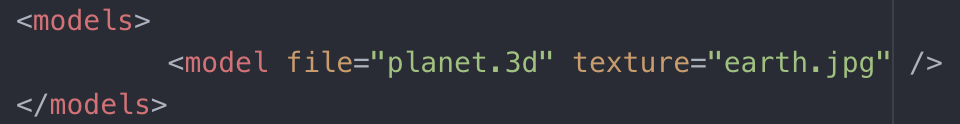
\includegraphics[scale=0.7]{xml_textura.png}
\caption{Textura para a Terra}
\label{img:textura_terra}
\end{figure}


\subsubsection{Funcionamento}
\label{sec:funcionamentot}

Ao fazer parsing do \textbf{XML} quando se encontra um parâmetro \textbf{"texture"}, o que se faz é aplicar a função \textbf{loadTexture} à imagem passada como parâmetro.

A função \textbf{loadTexture} tem como finalidade carregar a textura duma imagem (neste caso em 2D) e retornar uma um identificador dessa textura.

\begin{lstlisting}[language = C++ , frame = trBL , firstnumber = 1 , escapeinside={(*@}{@*)}]
int loadTexture(string s) {
    unsigned int t,tw,th;
    unsigned char *texData;
    unsigned int texID;

    ilInit();
    ilEnable(IL_ORIGIN_SET);
    ilOriginFunc(IL_ORIGIN_LOWER_LEFT);
    ilGenImages(1,&t);
    ilBindImage(t);
    ilLoadImage((ILstring) s.c_str());
    tw = ilGetInteger(IL_IMAGE_WIDTH);
    th = ilGetInteger(IL_IMAGE_HEIGHT);
    ilConvertImage(IL_RGBA, IL_UNSIGNED_BYTE);
    texData = ilGetData();
    glGenTextures(1,&texID);

    glBindTexture(GL_TEXTURE_2D,texID);
    glTexParameteri(GL_TEXTURE_2D,  GL_TEXTURE_WRAP_S,      GL_REPEAT);
    glTexParameteri(GL_TEXTURE_2D,  GL_TEXTURE_WRAP_T,      GL_REPEAT);
    glTexParameteri(GL_TEXTURE_2D,  GL_TEXTURE_MAG_FILTER,      GL_LINEAR_MIPMAP_LINEAR);
    glTexParameteri(GL_TEXTURE_2D,  GL_TEXTURE_MIN_FILTER, GL_LINEAR_MIPMAP_LINEAR);
    glTexImage2D(GL_TEXTURE_2D, 0, GL_RGBA, tw, th, 0, GL_RGBA, GL_UNSIGNED_BYTE, texData);
    glGenerateMipmap(GL_TEXTURE_2D);
    glBindTexture(GL_TEXTURE_2D, 0);

    return texID;

}
\end{lstlisting}

Após esta função terminar o identificador da textura é guardado na figura correspondente para mais tarde poder ser carregada.

\subsection{Engine}
\label{sec:enginet}

Finalmente no ciclo de rendering a textura é carregada tendo em conta o identificador previamente carregado na tarefa de parsing, da seguinte forma:

\begin{lstlisting}[language = C++ , frame = trBL , firstnumber = 1 , escapeinside={(*@}{@*)}]
	glBindTexture(GL_TEXTURE_2D, fig.textureId);

	.
	.
	.

	glBindBuffer(GL_ARRAY_BUFFER, fig.textures);
	glTexCoordPointer(2, GL_FLOAT, 0, 0);
\end{lstlisting}

A textura é então carregada tendo em conta o identificador anteriormente calculado, que se encontra em \textbf{fig.textureId}, e também o array das coordenadas de textura é carregado tendo em conta o identificador da VBO correspondente armazenado em \textbf{fig.textures}.



\section{Conclusão}
\label{sec:conclusao}

\end{document}
